\documentclass[plain]{beamer}
% Idioma: español
\usepackage[spanish,es-lcroman]{babel} % Características del idioma
\usepackage[utf8]{inputenc} % Acentos

%% Aspecto de página
%\usepackage[a4paper]{geometry} % Márgenes
%%\usepackage[left=4.72cm,right=4.72cm, top=4.4cm, bottom=4.21cm]{geometry} % Márgenes
%\usepackage{fancyhdr} % Headers
%\usepackage{parskip} % Espacio entre párrafos
%\usepackage{microtype} % Kerning y mejoras tipográficas
%\usepackage{pagecolor} % Color de fondo
%\usepackage{everypage} % \AddThispageHook {\tikz[remember picture,overlay] ... }
%
%% Columnas y tablas
%\usepackage{multicol}
%\usepackage{multirow}
%\usepackage{tabularx}
%\usepackage{tabu}
%\usepackage{diagbox} % Dividir una celda de un tabular
%\def\arraystretch{1}
%
%% Imágenes
\usepackage{graphicx}
%\usepackage{wrapfig}
\usepackage{caption}
\graphicspath{{img/}}
%
%% Símbolos
%\usepackage{mathtools} % \text, \overset, \underset
%\usepackage{amssymb} % \mathbb
%\usepackage{upgreek} % \uptheta
%\usepackage{amsthm} % QED
%\usepackage{marvosym} % \EUR
%
%% Formato
\usepackage{xcolor}
%\usepackage{soul} % \so, \st, \hl
%\usepackage{cancel} % \cancel, \bcancel, \xcancel, \cancelto
%\newcommand*\canceling[2][thin]{\tikz[baseline] \node [strike out,draw,anchor=text,inner sep=0pt,text=black,#1]{#2};}
%
%% Listas
%\usepackage{enumerate} % Numeración de listas
%\usepackage{outlines} % \0 \1 \2 \3 \4
%
%% Dibujos y gráficas
\usepackage{tikz}
%\usepackage{pgfplots}
\usetikzlibrary{shapes,arrows,arrows.meta,decorations.markings,shapes.misc,shapes.geometric,calc,pgfplots.groupplots}
%\pgfplotsset{compat=1.13}
%
%% Índices y títulos
%\addto\captionsspanish{\renewcommand{\contentsname}{Índice}}
%\usepackage{titlesec} % Formato de títulos
%%\usepackage{minitoc} % Índices de secciones
%\usepackage{hyperref} % Links
%\hypersetup{colorlinks}
%
%% Otros
%\usepackage[spanish,colorinlistoftodos,obeyDraft]{todonotes} % ToDo
%\usepackage{pdfpages} % Incluir PDFs
\usepackage{qrcode} % QR
%\usepackage{chemfig} % Química
%\usepackage{wasysym} % Notas musicales
%
%\usepackage[acronym]{glossaries} % Siglas y glosario
%\usepackage{acronym} % Acrónimos

% Código
\usepackage{listings}
\lstset{
	inputencoding=utf8,
	extendedchars=true,
	literate=%
	{á}{{\'a}}1
	{é}{{\'e}}1
	{í}{{\'i}}1
	{ó}{{\'o}}1
	{ú}{{\'u}}1
	{Á}{{\'A}}1
	{É}{{\'E}}1
	{Í}{{\'I}}1
	{Ó}{{\'O}}1
	{Ú}{{\'U}}1
	{ñ}{{\~n}}1
	{Ñ}{{\~N}}1
	{¿}{{>}}1
	{¡}{{<}}1
}
\lstset{ %
	backgroundcolor=\color{white},
	basicstyle=\footnotesize,
	breakatwhitespace=false,
	breaklines=true,
	extendedchars=true,              
	frame=single,          
	language=Python,                
	numbers=none,  
	rulecolor=\color{black},        
	showspaces=false,               
	showstringspaces=false,          
	showtabs=false,
	tabsize=4,
	morekeywords={},
	columns=flexible,    
	escapechar=¬,
}
%\lstset{
%language=[Latex]Tex,
%%
%basicstyle=\footnotesize\sffamily,
%keywordstyle=\footnotesize\sffamily,
%identifierstyle=\footnotesize\sffamily,
%commentstyle=\footnotesize\sffamily,
%stringstyle=\footnotesize\sffamily,
%escapechar=¬,
%%		
%numberstyle=\footnotesize\sffamily,%\ttfamily\tiny\color[gray]{0.3},
%numbers=left,
%stepnumber=2,
%numbersep=15pt,
%%
%columns=flexible,
%showstringspaces=false,
%tabsize=4,
%}

%% Apéndices
%\newcommand{\apendices}
%{\section*{Apéndices}%
%	\addcontentsline{toc}{section}{Apéndices}
%	\setcounter{section}{0}%
%	\setcounter{subsection}{0}%
%	\renewcommand\thesection{\Alph{section}}%
%}
%
%\newenvironment{changemargin}[2]{%
%	\begin{list}{}{%
%			\setlength{\topsep}{0pt}%
%			\setlength{\leftmargin}{#1}%
%			\setlength{\rightmargin}{#2}%
%			\setlength{\listparindent}{\parindent}%
%			\setlength{\itemindent}{\parindent}%
%			\setlength{\parsep}{\parskip}%
%		}%
%		\item[]
%}
%{\end{list}}
\setbeamertemplate{navigation symbols}{}

\usepackage{fontspec}
\newfontfamily\emojifont{Twitter Color Emoji}

\usepackage[normalem]{ulem}
\newcommand{\soutt}[1]{%
	\renewcommand{\ULthickness}{2pt}%
	\sout{#1}%
	\renewcommand{\ULthickness}{.4pt}%
}

\usepackage{fancybox}
\makeatletter
\newenvironment{CenteredBox}{% 
	\begin{Sbox}}{%
	\end{Sbox}\centerline{\parbox{\wd\@Sbox}{\TheSbox}}}%
\makeatother

\newcommand{\ee}[1]{{\emojifont \char"#1{}}}

\begin{document}

\begin{frame}
\begin{center}	
	{\LARGE Análisis de\\
	\soutt{Complejidad} Simplicidad\\[5pt]
	de Algoritmos}\\[20pt]

	\resizebox{2cm}{1.25cm}{\ee{1F570}}\\[30pt]
 
	Celia Rubio Madrigal
\end{center}
\end{frame}

\begin{frame}
	
	\textbf{Definición 1.1. (Algoritmo reticente)}\\[20pt]
	
	$A$ es un algoritmo reticente para el problema $P$ sí, y solo sí,~\hyperlink{uno}{[1]}
	
	\[(\forall M)\ \mathcal{G}(A,t,M,P) \implies \bigwedge\limits_{o\in\mathcal{I}}\mathcal{E}(M,o)\]
	
	donde $t$ es el tiempo, $\mathcal{G}(A,t,M,P)$ es el predicado
	\begin{center}
		\it``$A$ gasta un tiempo $t$ de la manera $M$ mientras resuelve $P$'',
	\end{center}
	$\mathcal{I}$ es el conjunto de observadores ingenuos
	y $\mathcal{E}(M,o)$ es el predicado
	\begin{center}
		\it``$M$ es suficientemente artificiosa como para engañar a $o$''.
	\end{center}
\end{frame}

\begin{frame}
	\ \\[20pt]
	\textbf{Ejemplo 1.1.} La búsqueda de la llave correcta a la hora de abrir una cerradura.\\[15pt]
	
	\textbf{Ejemplo 1.2.} El recorrido de grafos en la Odisea de Homero.\\[15pt]
	
	\textbf{Ejemplo 1.3.} La vuelta atrás.\\[15pt]
	
	\textbf{Ejemplo 1.4.} La resolución de buscaminas de María.\\[15pt]

	\begin{center}
		\bigskip
		
		{\Huge\ee{1F36C}}\\
		{\color{white}respeta}
	\end{center}
\end{frame}


\begin{frame}
\begin{center}
	\bigskip
	\begin{tikzpicture}[xscale=-1]
		\draw[{<[length=3mm,width=5mm]}-{>[length=3mm,width=5mm]}] 
		(7,-0.5) node[below=20pt] {\Huge\resizebox{1.5cm}{1cm}{\ee{26A1}\ee{26A1}}} --
		(0,-0.5)  node[below=20pt] {
\includegraphics[height=1cm]{bbs}};
		
		\visible<1>{\node at (6,2.75) {\rotatebox{0}{Merge}};}
		\visible<1>{\node at (5.25,2) {\rotatebox{0}{Bubble}};}
		\visible<1>{\node at (6,1.25) {\rotatebox{0}{Quick}};}
		
		\visible<1->{\node at (7,1.25) {\ee{270B}};}
		\visible<1->{\node at (7,2) {\ee{270B}};}
		\visible<1->{\node at (7,2.75) {\ee{270B}};}
		\begin{scope}
			\visible<2->{
				\node at (1,2.75) {\ \href{run:bogo.mp4}{\ee{1F4F9}} Bogo};
				\node at (1.4,2) {\rotatebox{0}{\ee{2665}}};
				\node at (1.4,1.25) {\rotatebox{0}{\ee{2666}}};
				\node at (0.6,2) {\rotatebox{0}{\ee{2663}}};
				\node at (0.6,1.25) {\rotatebox{0}{\ee{2660}}};
			}
		\end{scope}
	\end{tikzpicture}\\	
	{\color{white}loss}
\end{center}
\end{frame}

\begin{frame}[fragile]
\begin{center}
	{\LARGE\textbf{Algoritmo 1.1. (Bogo)} \ee{1F0CF}}\\[30pt]
\begin{lstlisting}
    import random

    def is_sorted(L) :
        return all(L[i] <= L[i+1] for i in range(len(L)-1))

    def bogo(L) :
        while not is_sorted(L) :
            random.shuffle(L)
    return L
\end{lstlisting}
\end{center}
\end{frame}

\begin{frame}[fragile]
\begin{center}
	{\LARGE\textbf{Algoritmo 1.1. (Bogo)} \ee{1F0CF}}\\[10pt]
	(Versión probabilista \textit{Las Vegas})
\end{center}
\begin{columns}
\begin{column}{0.5\textwidth}
\begin{center}
\begin{lstlisting}
    def LV(x, y) :
        y = x
        random.shuffle(y)
        return is_sorted(y)

    def repetirLV(x) :
        y = x
        exito = False
        while not exito :
            LV(x, y, exito)
        return y
\end{lstlisting}
\end{center}
\end{column}
\begin{column}{0.5\textwidth}
	Si |x| = n:
\begin{center}
	\setbeamertemplate{itemize item}{\color{black}$\blacktriangleright$}
	\begin{itemize}
		\item p(x) = $\dfrac{1}{\text{n}!}$
		\item e(x) = f(x) = n
		\item t(x) = e(x) + $\dfrac{1-\text{p(x)}}{\text{p(x)}}$f(x) = n + (n!$- 1$)n = n$\cdot$n!
	\end{itemize}
\end{center}
\end{column}
\end{columns}
\end{frame}

\begin{frame}
\begin{center}
	{\LARGE\textbf{Algoritmo 1.1. (Bogo)} \ee{1F0CF}}\\[20pt]
\end{center}
	
	\qquad\qquad\qquad\qquad{\LARGE\ee{231B}}\quad Tiempo esperado: O(n$\cdot$n!)
	\\[20pt]
	
	\qquad\qquad\qquad\qquad{\LARGE\ee{1F51C}}\quad Caso mejor: ¡ O(n) !
	\\[20pt]

	\qquad\qquad\qquad\qquad{\LARGE\ee{267E}}\quad Caso peor: ¡¡ O($\infty$) !!
	\\[20pt]

	\qquad\qquad\qquad\qquad{\LARGE\ee{1F500}}\quad ¿Generador aleatorio?
\end{frame}

\begin{frame}[fragile]
\begin{center}
	{\LARGE\textbf{Arreglo 1.1.} (\ee{1F500} y \ee{267E})}
	\\[10pt]
	{En vez de permutar aleatoriamente,\\
		recorremos las permutaciones una a una.}
	\\[30pt]
	
	\begin{CenteredBox}
	\begin{lstlisting}[linewidth=0.5\textwidth]
    from itertools import permutations
	
    def bad(L) :
        P = permutations(L)
        for X in P :
            if is_sorted(X) :
            return X
        return
\end{lstlisting}
\end{CenteredBox}
\end{center}
\end{frame}

\begin{frame}[fragile]
\begin{center}
	{\LARGE\textbf{Arreglo 1.2.} (\ee{1F51C})}
	\\[10pt]
	{En vez de recorrer las permutaciones,\\
		generamos todas ellas al principio.}
	\\[30pt]
	
	
\begin{CenteredBox}
	\begin{lstlisting}[linewidth=0.5\textwidth]
    def worse(L) :
        P = list(permutations(L))
        for X in P :
            if is_sorted(X) :
            return X
        return
\end{lstlisting}

\end{CenteredBox}
\end{center}
\end{frame}

\begin{frame}
\begin{center}	
	{\LARGE\textbf{Arreglo 1.3.} (\ee{231B})}
	\\[20pt]
	
	\pause{La permutación correcta es la lexicográficamente\\
	\textbf{menor} de ellas $\implies$ podemos \textbf{ordenarlas}\\
	y tomar la primera permutación.~\hyperlink{dos}{[2]}}\\[30pt]

	\pause{\bf\LARGE¡Ordenación recursiva!}
\end{center}
\end{frame}

\newcommand{\cart}[1]{node[draw,rectangle,rounded corners] {{#1}}}
\newcommand{\baraj}[2]{%
	\draw[rounded corners] (-0.375, -0.375) rectangle (0.875, 0.375) {};
	\draw (0,0) \cart{#1};
	\draw (0.5,0) \cart{#2};
}
\begin{frame}
\begin{center}
	\begin{tikzpicture}
	\begin{scope}[yshift=-0.25cm]
	\baraj{2}{1}
	\end{scope}
	
	\begin{scope}[xshift=-1cm,yshift=-1.5cm]
	\baraj{2}{1}
	\end{scope}
	\begin{scope}[xshift=1cm,yshift=-1.5cm]
	\baraj{1}{2}
	\end{scope}
	
	\begin{scope}[xshift=-3cm,yshift=-3cm]	
	\draw[rounded corners] (-0.65, -0.65) rectangle (2.65, 0.65) {};
	\baraj{2}{1}
	\end{scope}
	\begin{scope}[xshift=-1.5cm,yshift=-3cm]
	\baraj{1}{2}
	\end{scope}	
	\begin{scope}[xshift=1.5cm,yshift=-3cm]
	\draw[rounded corners] (-0.65, -0.65) rectangle (2.65, 0.65) {};
	\baraj{1}{2}
	\end{scope}
	\begin{scope}[xshift=3cm,yshift=-3cm]
	\baraj{2}{1}
	\end{scope}
	
	
	\begin{scope}[xshift=1.5cm,yshift=-5cm]	
	\draw[rounded corners] (-0.65, -0.65) rectangle (2.65, 0.65) {};
	\baraj{2}{1}
	\end{scope}
	\begin{scope}[xshift=3cm,yshift=-5cm]
	\baraj{1}{2}
	\end{scope}
	
	\begin{scope}[xshift=-3cm,yshift=-5cm]
	\draw[red,rounded corners] (-0.65, -0.65) rectangle (2.65, 0.65) {};	
	\draw[red,rounded corners] (-0.375, -0.375) rectangle (0.875, 0.375) {};
	\draw (0,0) \cart{1};
	\draw (0.5,0) \cart{2};
	\end{scope}
	\begin{scope}[xshift=-1.5cm,yshift=-5cm]
	\baraj{2}{1}
	\end{scope}
	
	\draw[-{Latex[length=3mm,width=3mm]}] (-2,-3.5) -- (2.5,-4.25);
	\draw[-{Latex[length=3mm,width=3mm]}] (2.5,-3.5) -- (-2,-4.25);
	\end{tikzpicture}
\end{center}
\end{frame}


\begin{frame}[fragile]
\begin{center}
	{\LARGE\textbf{Algoritmo 1.2. (Worst Sort)} \ee{1F501}}\\[20pt]
\end{center}
\begin{columns}
	\begin{column}{0.5\textwidth}
		\begin{center}
\begin{lstlisting}
    def multi(L, N) :
        if N == 0 :
            return sorted(L)
        P = list(permutations(L))
        P = multi(P, N-1)
        return P[0]
            
    def worst(L) :
        return multi(L, cota(len(L)))
\end{lstlisting}
		\end{center}
	\end{column}
	\begin{column}{0.5\textwidth}
		\begin{center}
			\setbeamertemplate{itemize item}{\color{black}$\blacktriangleright$}
			\begin{itemize} \Large
				\item $\Omega\big($%
				n$!!\overset{\text{f(n)}}{\cdots}!!$%
				$\big)$
				\bigskip\smallskip
				\visible<2->{\item $\lim\limits_{\text{n}\to\infty}\dfrac{\text{\ee{1F171}\ee{1F171}}}{\big(\text{n}!!\overset{\text{f(n)}}{\cdots}!!\big)}=\infty$}
			\end{itemize}		
		{\color{white}esp}
		\end{center}
	\end{column}
\end{columns}
\end{frame}

\begin{frame}
	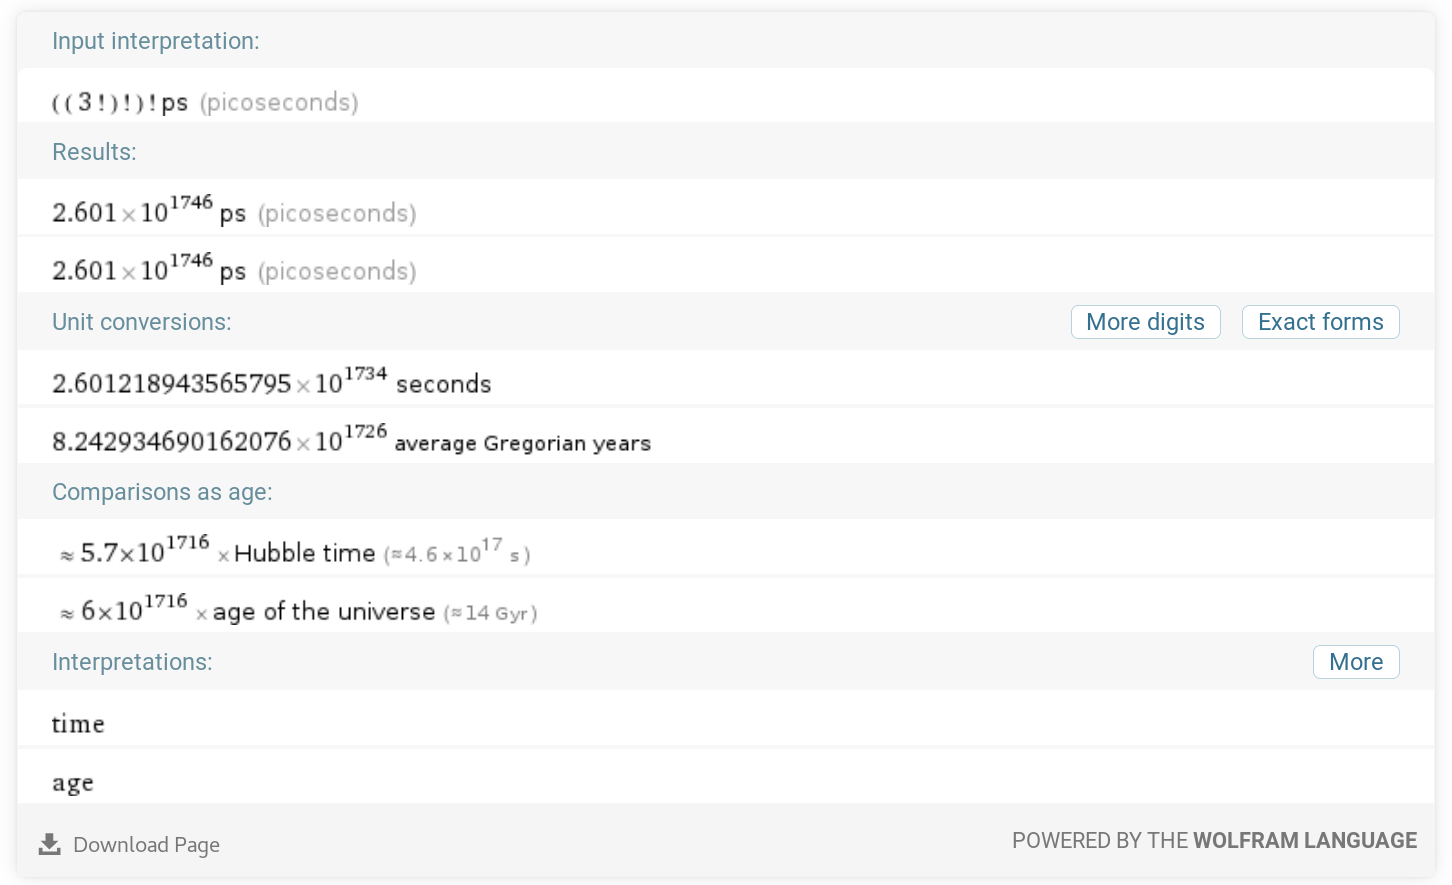
\includegraphics[width=\columnwidth]{picoseconds}
\end{frame}

\begin{frame}\Huge
\begin{center}
	\resizebox{6.75cm}{2cm}{\ee{2716} \ \ee{1F3F3}}\\[20pt]
	(multiplica y ríndete)
\end{center}
\end{frame}

\begin{frame}
\begin{center}
	{\Huge \ee{2716} \ee{1F3F3}}\\
	(multiplica y ríndete)\\
[10pt]
	
	
	\begin{tikzpicture}[scale=0.9]
		\large
\visible<1->{
	\node (1) at (0,0) {sort[0 : n)};
}
\visible<2->{
	\node (2) at (-2,-1.25) {\alert<5->{sort[0 : $\frac{\text{n}}{\text{2}}$)}};
		\draw[-{Latex[length=2mm,width=2mm]}] (1) -- (2);
		\visible<5->{\draw[red,smooth,-{Latex[length=2mm,width=2mm]}] (2)
		to[out=180,in=170] (1);}
	\node (3) at (2,-1.25) {\alert<5->{sort[$\frac{\text{n}}{\text{2}}$ : n)}};
		\draw[-{Latex[length=2mm,width=2mm]}] (1) -- (3);
		\visible<5->{\draw[red,smooth,-{Latex[length=2mm,width=2mm]}] (3)
		to[out=0,in=10] (1);}
}
\visible<3->{
	\draw[-{Latex[length=2mm,width=2mm]}] (2) -- (-1,-2.25);
	\draw[-{Latex[length=2mm,width=2mm]}] (3) -- (2,-2.25);
	\node (4) at (0,-2.75) {max( max[0 : $\frac{\text{n}}{\text{2}}$) , max[$\frac{\text{n}}{\text{2}}$ : n) )};
}
\visible<4->{
	\draw[-{Latex[length=2mm,width=2mm]}] (4) -- (1.5,-4);
	\node (5) at (0,-4.5) {\alert<5->{sort[0 : n-1)} + [n-1)};
		\visible<5->{\draw[red,smooth,-{Latex[length=2mm,width=2mm]}] (5)
		to[out=180,in=-5] (1);}
}
	\end{tikzpicture}
	
\end{center}
\end{frame}


\begin{frame}[fragile]
\begin{center}
	{\LARGE\textbf{Algoritmo 1.3. (Slow Sort)} \ee{26A0}}\\[30pt]
\end{center}
\begin{center}
\begin{CenteredBox}
\begin{lstlisting}[linewidth=0.5\textwidth]
    def slow(L, i, j) :
        if i >= j :
            return
        m = (i+j) // 2 
        slow(L, i, m)
        slow(L, m + 1, j)
        if L[j] < L[m] :
            L[j], L[m] = L[m], L[j]
        slow(L, i, j-1)
        return L
\end{lstlisting}
\end{CenteredBox}
\end{center}
\end{frame}

\section{}
\begin{frame}\large
	\begin{center}
		{\LARGE \ee{1F516} \textbf{Referencias} \ee{1F516}}
	\end{center}
	\begin{enumerate}
		\item[\color{black}[1\!\!\!]] Broder, A., Stolfi, J.\phantomsection\label{uno}\\
		\href{https://www.mipmip.org/tidbits/pasa.pdf}
		{\textit{Pessimal Algorithms and Simplexity Analysis}}, 1984.
		\item[\color{black}[2\!\!\!]] Lerma, M. A.\phantomsection\label{dos}\\
		\href{https://sites.math.northwestern.edu/~mlerma/papers/inefficient_algorithms.pdf}
		{\textit{How inefficient can a sort algorithm be?}} 2014.
	\end{enumerate}
\begin{figure}[!h]
	\qrcode{https://gitlab.com/celiaru/simplicidad}
	\caption*{\href{https://gitlab.com/celiaru/simplicidad}{Código de las diapositivas} (C++, Python)}
\end{figure}
\end{frame}

\end{document}
